\documentclass[twoside,11pt,ShortChapTitles]{BYUTextbook}

\usepackage{soul}
\renewcommand{\vec}[1]{\ensuremath{\mathbf{#1}}}
\newcounter{dummy}
\newcommand{\labsection}[1]{\refstepcounter{dummy}\addcontentsline{toc}{section}{#1}\section*{#1}}
\usepackage{siunitx}
\sisetup{round-mode = figures,
  round-precision = 3, scientific-notation=true}

\begin{document}

\frontmatter

 \thispagestyle{empty}
 \begin{adjustwidth}{}{-1.5in}
 \centering
 {\huge PH150: Introduction to experimental and numerical techniques
   in Physics}
 \vskip1.5truein

    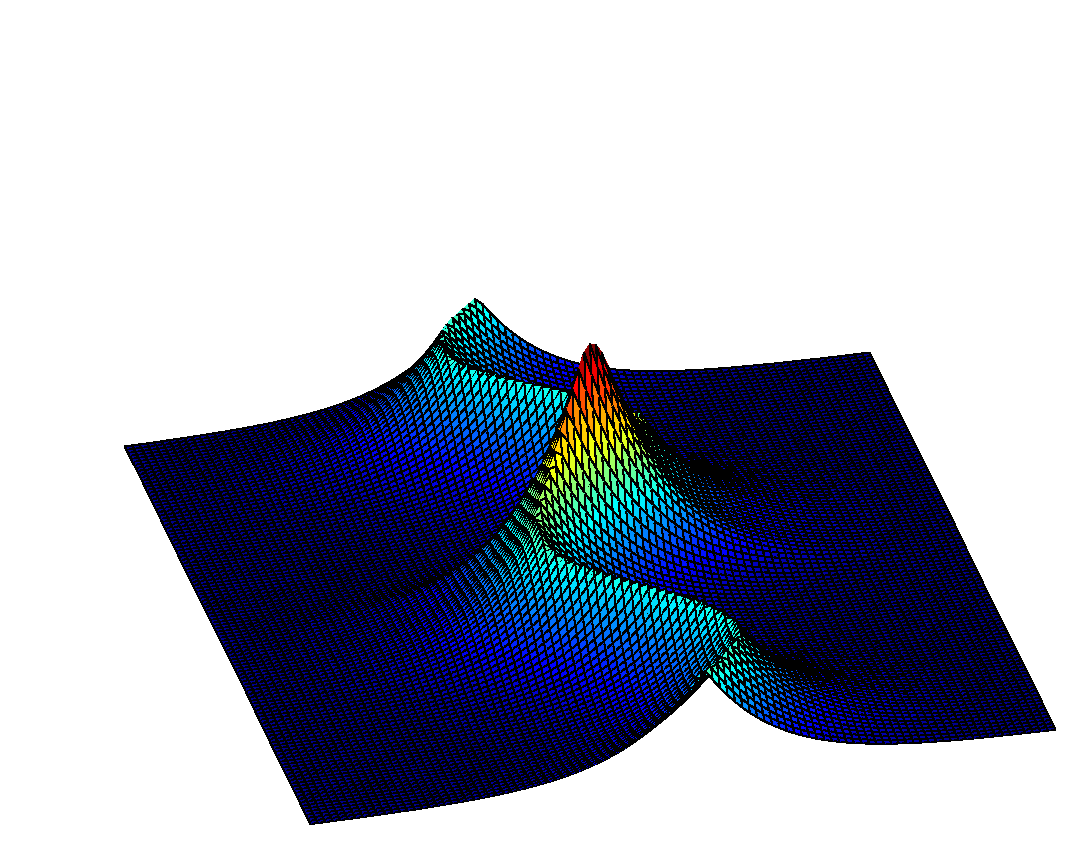
\includegraphics[scale=.80]{matlabcover}

\vskip1truein
Lance J.\ Nelson

\vskip.4truein
Department of Physics
\end{adjustwidth}

\cleardoublepage
\thispagestyle{empty}

 \begin{adjustwidth}{}{-1.5in}
 \centering
 \vspace*{1in}
 \large
 {\huge PH150: Introduction to experimental and numerical techniques
   in Physics}
 \vskip.4truein

 Lance J.\ Nelson
 \bigskip

 Department of Physics

 \bigskip
 Brigham Young University--Idaho

 \vfill


 {\footnotesize $\copyright$ 2017 Lance J.\ Nelson
               Brigham Young University--Idaho}

 \vskip.5truein
 {\footnotesize \emph{Last Revised: \today}}
 \normalsize

 \end{adjustwidth}

\cleardoublepage

\chapter*{Preface}

This is a lab notebook intended to give you experience with
uncertainty analysis, experimental methods, and numerical methods in
physics.  All text with a bold P designation (\textbf{P1.1} for
example) indicates a task to be done.  Usually this will involve
writing something in your lab notebook.  Please be as complete and
neat as possible.

Any tasks that requires a computer will be done using the Python
programming language.  You can obtain a free copy of Python \href{https://store.enthought.com/downloads/}{here}.  
Any computer code that you create should be uploaded to the Google
Drive folder provided.

There is a companion book to this one entitled, ``Introduction to
Python''.  It is intended to help you learn to use Python to do the
tasks contained herein.  


 \cleardoublepage \phantomsection
 \addcontentsline{toc}{chapter}{Table of Contents}
\tableofcontents

\mainmatter

\chapter*{Review}
\addcontentsline{toc}{chapter}{Review}

If you are like most students, loops and logic gave you trouble in
330. We will be using these programming tools extensively this
semester, so you may want to review and brush up your skills a bit.
Here are some optional problems designed to help you remember your
loops and logic skills. You will probably need to use online help
(and you can ask a TA to explain things in class too).

\begin{enumerate}
\subprob \index{For loop} \index{Loops!for} Write a {\tt for}
    loop that counts by threes starting at 2 and ending at 101.
    Along the way, every time you encounter a multiple of 5 print
    a line that looks like this (in the printed line below it
    encountered the number 20.)
\begin{Verbatim}
fiver: 20
\end{Verbatim}
    You will need to use the commands {\tt for}, {\tt mod}, and
    {\tt fprintf}, so first look them up in online help.

\subprob Write a loop that sums the integers from 1 to $N$, where
    $N$ is an integer value that the program receives via the
    {\tt input} command. Verify by numerical experimentation that
    the formula
    \[
        \sum_{n=1}^N n = \frac{N(N+1)}{2}
    \]
    is correct

\subprob For various values of $x$ perform the sum
    \[
        \sum_{n=1}^{1000} n x^n
    \]
    with a {\tt for} loop and verify by numerical experimentation
    that it only converges for $|x| < 1$ and that when it does
    converge, it converges to $x/(1-x)^2$.

\index{While loop} \index{Loops!while}
\subprob Redo (c) using a {\tt while} loop (look it up in online
    help.) Make your own counter for $n$ by using $n=0$ outside
    the loop and $n=n+1$ inside the loop. Have the loop execute
    until the current term in the sum, $n x^n$ has dropped below
    $10^{-8}$. Verify that this way of doing it agrees with what
    you found in (c).

\subprob Verify by numerical experimentation with a {\tt while}
    loop that
    \[
        \sum_{n=1}^{\infty} \frac{1}{n^2} = \frac{\pi^2}{6}
    \]
    Set the {\tt while} loop to quit when the next term added to
    the sum is below $10^{-6}$.

\subprob Verify, by numerically experimenting with a {\tt for}
    loop that uses the {\tt break} command (see online help) to
    jump out of the loop at the appropriate time, that the
    following infinite-product relation is true:
    \[
        \prod_{n=1}^{\infty} \left( 1 + \frac{1}{n^2} \right)
        = \frac{ \sinh{\pi} }{ \pi }
    \]

\subprob \index{Iteration} \index{Successive substitution} Use a
    {\tt while} loop to verify that the following three iteration
    processes converge. (Note that this kind of iteration is
    often called successive substitution.) Execute the loops
    until convergence at the $10^{-8}$ level is achieved.
    \[
        x_{n+1} = e^{-x_n}~~~~;~~~~
        x_{n+1} = \cos{x_n}~~~~;~~~~
        x_{n+1} = \sin{2 x_n}
    \]
    Note: iteration loops are easy to write. Just give $x$ an
    initial value and then inside the loop replace $x$ by the
    formula on the right-hand side of each of the equations
    above. To watch the process converge you will need to call
    the new value of $x$ something like {\tt xnew} so you can
    compare it to the previous $x$.

    Finally, try iteration again on this problem:
    \[
        x_{n+1} = \sin{3 x_n}
    \]
    Convince yourself that this process isn't converging to
    anything. We will see in Lab~\ref{Lab:10} what makes the
    difference between an iteration process that converges and
    one that doesn't.
\end{enumerate}

\mainmatter

\pagestyle{fancy}
\renewcommand{\chaptermark}[1]{\markboth{Computational Physics 385}{\chaptername \ \thechapter \ \ #1}}

\chapter[Grids and Numerical Derivatives]{Grids and Numerical Derivatives}
\label{ch:grids}
%\addcontentsline{toc}{chapter}{Grids and Derivatives}

When we solved differential equations in Physics 295 we were usually
moving something forward in time, so you may have the impression that
differential equations always ``flow.'' This is not true. If we solve
a spatial differential equation, for instance, like the one that
gives the shape of a chain draped between two posts, the solution
just sits in space; nothing flows. Instead, we choose a small spatial
step size (think of each individual link in the chain) and we seek to
find the correct shape by somehow finding the height of the chain at
each link.

In this course we will be solving partial differential equations,
which usually means that the desired solution is a function of both
space $x$, which just sits, and time $t$, which flows.
\index{Spatial grids} And when we solve problems like this we will
be using {\it spatial grids}, to represent the $x$-part that
doesn't flow. You have already used grids in Python to do simple
jobs like plotting functions and doing integrals numerically.
Before we proceed to solving partial differential equations, let's
spend some time getting comfortable working with spatial grids.

\marginfig[-1in]{chapters/f01Grids}{\label{f01Grids}Three common spatial grids}

\labsection{Spatial grids}

Figure~\ref{f01Grids} shows a graphical representation of three
types of spatial grids for the region $0 \le x \le L$.  We divide
this region into spatial \emph{cells} (the spaces between vertical
lines) and functions are evaluated at $N$ discrete \emph{grid
points} (the dots). In a \emph{cell-edge} grid,\index{Cell-edge
grid}\index{Grids!cell-edge} the grid points are located at the
edge of the cell.  In a \emph{cell-center} grid,\index{Cell-center
grid}\index{Grids!cell-center} the points are located in the middle
of the cell.  Another useful grid is a cell-center grid with {\it
ghost points}.\index{Ghost points} The ghost points (unfilled dots)
are extra grid points on either side of the interval of interest
and are useful when we need to consider the derivatives at the edge
of a grid.

\begin{enumerate}
\prob \label{P:1.1}
\begin{enumerate}
\subprob \label{P:1.1a} Make a Python script that creates a
    cell-edge spatial grid in the variable {\tt x} as
    follows: \marginfig{chapters/f01p1a}{Plot from \ref{P:1.1a}}
\begin{Verbatim}
from numpy import arange  # Import the needed function
N=100             % the number of grid points
a=0
b=pi          % the left and right bounds
h=(b-a)/(N-1)     % calculate the step size
x=arange(a,b,h)           % build the grid
\end{Verbatim}
    Plot the function $y(x) = \sin(x) \sinh(x)$ on this grid.
    Explain the relationship between the number of cells and
    the number of grid points in a cell-edge grid and why you
    divide by {\tt (N-1)} when calculating {\tt h}. Then
    verify that the number of points in this $x$-grid is $N$
    (using Python's {\tt len} command).

\subprob \label{P:1.1b} Explain the relationship between the
    number of cells and the number of grid points in a
    cell-center grid and decide how you should modify the
    line that calculates {\tt h} in (a) to get the correct
    spacing for a cell-center grid.

    \marginfig{chapters/f01p1b}{Plot from \ref{P:1.1b}}

    Now write a script like the one in part (a) to build a cell-center
    grid over the interval $0 \le x \le 2$ with $N=5000$. Evaluate the
    function $f(x)=\cos{x}$ on this grid and plot this function. Then
    estimate the area under the curve by summing the products of the
    centered function values $f_j$ with the widths of the cells $h$
    like this (midpoint integration rule):
\begin{Verbatim}
sum(f)*h;
\end{Verbatim}

    Verify that this result is quite close to the exact
    answer obtained by integration:
    \[
        A=\int_0^2 \cos{x} ~dx.
    \]

\subprob Build a cell-center grid with ghost points over the
    interval $0 \le x \le \pi/2$ with 500~cells (502 grid
    points), and evaluate the function $f(x)=\sin{x}$ on this
    grid.  Now look carefully at the function values at the
    first two grid points and at the last two grid points.
    The function $\sin{x}$ has the property that $f(0)=0$ and
    $f'(\pi/2)=0$. The cell-center grid doesn't have points
    at the ends of the interval, so these boundary conditions
    on the function need to be enforced using more than one
    point. Explain how the ghost points can be used in
    connection with interior points to specify both
    function-value boundary conditions and derivative-value
    boundary conditions.
\end{enumerate}
\end{enumerate}

%Python has a convenient command {\tt linspace} for building one
%dimensional grids.  The syntax for building a grid is
%\begin{Verbatim}
%x = linspace(a,b,N);
%\end{Verbatim}
%where {\tt a} is the $x$ position of the first point in the grid,
%{\tt b} is the $x$-position of the last point in the grid, and {\tt
%N} is the number of grid points.  This method doesn't give you the
%grid spacing back, but you can always calculate it by subtraction:
%\begin{Verbatim}
%h = x(2) - x(1);
%\end{Verbatim}
%Depending on what you choose for {\tt a} and {\tt b}, {\tt linspace}
%can give you either cell-edge or cell-center grids.

\labsection{Interpolation and extrapolation}
\index{Interpolation} \index{Extrapolation}

Grids only represent functions at discrete points, and there will be
times when we want to find good values of a function {\it between}
grid points (interpolation) or \emph{beyond} the last grid point
(extrapolation). We will use interpolation and extrapolation
techniques fairly often during this course, so let's review these
ideas.

\marginfig{chapters/f01Linear}{The line defined by two points can be used to
interpolate between the points and extrapolate beyond the points.}

The simplest way to estimate these values is to use the fact that two
points define a straight line. For example, suppose that we have
function values $(x_1,y_1)$ and $(x_2,y_2)$. The formula for a
straight line that passes through these two points is
\begin{equation} \label{eq:linear}
    y-y_1 = \frac{ (y_2-y_1) }{ (x_2-x_1) } (x-x_1)
\end{equation}
Once this line has been established it provides an approximation to
the true function $y(x)$ that is pretty good in the neighborhood of
the two data points. To linearly interpolate or extrapolate we simply
evaluate Eq.~(\ref{eq:linear}) at $x$ values between or beyond $x_1$
and $x_2$.

\begin{enumerate}
\prob \label{P:1.3} Use Eq.~(\ref{eq:linear}) to do the following
    special cases:

\begin{enumerate}
\subprob Find an approximate value for $y(x)$ halfway between
    the two points $x_1$ and $x_2$. Does your answer make
    sense?

\subprob Find an approximate value for $y(x)$ 3/4 of the way
    from $x_1$ to $x_2$. Do you see a pattern?

\subprob If the spacing between grid points is $h$ (i.e.
    $x_2-x_1=h$), show that the linear extrapolation formula
    for $y(x_2+h)$ is
    \begin{equation}\label{eq:linExtrap}
        y(x_2+h) = 2 y_2 - y_1
    \end{equation}
    This provides a convenient way to estimate the function
    value one grid step beyond the last grid point.  Also
    show that
    \begin{equation}\label{eq:linExtraphalf}
        y(x_2+h/2) = 3 y_2 / 2 - y_1 / 2 .
    \end{equation}
    We will use both of these formulas during the course.
\end{enumerate}
\end{enumerate}

\marginfig{chapters/f01Quadratic}{Three points define a parabola that can be
used to interpolate between the points and extrapolate beyond the
points.}

A fancier technique for finding values between and beyond grid points
is to use a parabola instead of a line. It takes three data points to
define a parabola, so we need to start with the function values
$(x_1,y_1)$, $(x_2,y_2)$, and $(x_3,y_3)$. The general formula for a
parabola is
\begin{equation}\label{eq:Parabola}
    y=a + bx + cx^2
\end{equation}
where the coefficients $a$, $b,$ and $c$ need to be chosen so that
the parabola passes through our three data points. To determine these
constants, you set up three equations that force the parabola to
match the data points, like this:
\begin{equation}\label{eq:ParabolaSet}
    y_j = a + bx_j + cx_j^2
\end{equation}
with $j=1,2,3$, and then solve for $a$, $b$, and $c$.

\begin{enumerate}
\prob \label{P:1.4} Use Eq.~(\ref{eq:ParabolaSet}) to create a
    set of three equations in Mathematica. For simplicity, assume
    that the points are on an evenly-spaced grid and set
    $x_2=x_1+h$ and $x_3=x_1+2h$.  Solve this set of equations to
    obtain some messy formulas for $a$, $b$, and $c$ that involve
    $x_1$ and $h$. Then use these formulas to solve the following
    problems:

\begin{enumerate}

\subprob Estimate $y(x)$ half way between $x_1$ and $x_2$,
    and then again halfway between $x_2$ and $x_3$. Do you
    see a pattern? (You will need to simplify the answer that
    Mathematica spits out to see the pattern.)

\subprob Show that the quadratic extrapolation formula for
    $y(x_3+h)$ (i.e. the value one grid point beyond $x_3$)
    is
    \begin{equation}\label{eq:quadExtrap}
        y(x_3+h) = y_1 - 3 y_2 + 3 y_3
    \end{equation}
    Also find the formula for $y(x_3+h/2)$.
\end{enumerate}
\end{enumerate}


\labsection{Derivatives on grids}
\index{Derivatives, first and second}
\index{Forward difference formula}

This is a course on partial differential equations, so we will
frequently need to calculate derivatives on our grids. In your
introductory calculus book, the derivative was probably introduced
using the {\it forward difference} formula
\begin{equation}\label{eq:forwarddiff}
     f'(x) \approx \frac{f(x+h)-f(x)}{h} .
\end{equation}
The word ``forward'' refers to the way this formula reaches forward
from $x$ to $x+h$ to calculate the slope. The exact derivative
represented by Eq.~(\ref{eq:forwarddiff}) in the limit that $h$
approaches zero.  However, we can't make $h$ arbitrarily small when
we represent a function on a grid because (i) the number of cells
needed to represent a region of space becomes infinite as $h$ goes to
zero; and (ii) computers represent numbers with a finite number of
significant digits so the subtraction in the numerator of
Eq.~(\ref{eq:forwarddiff}) loses accuracy when the two function
values are very close. But given these limitation we want to be as
accurate as possible, so we want to use the best derivative formulas
available. The forward difference formula isn't one of them.

\marginfig{chapters/f01FiniteDifference}{The forward and centered difference
formulas both approximate the derivative as the slope of a line
connecting two points. The centered difference formula gives a more
accurate approximation because it uses points before and after the
point where the derivative is being estimated. (The true derivative
is the slope of the dotted tangent line).}

The best first derivative formula that uses only two function values
is usually the {\it centered difference} formula: \index{Centered
difference formula}
\begin{equation}\label{eq:CenteredDiff}
    f'(x) \approx \frac{f(x+h)-f(x-h)}{2h} .
\end{equation}
It is called ``centered'' because the point $x$ at which we want the
slope is centered between the places where the function is evaluated.
The corresponding centered second derivative formula is \index{Second
derivative}
\begin{equation}\label{eq:seconderivative}
    f''(x) \approx {f(x+h)-2 f(x)+f(x-h) \over h^2}
\end{equation}
You will derive both of these formulas a little later, but for now we
just want you to understand how to use them.

Python's colon operator provides a compact way to evaluate
Eqs.~(\ref{eq:CenteredDiff}) and (\ref{eq:seconderivative}) on a
grid.  If the function we want to take the derivative of is stored in
an array {\tt fp}, we can calculate the centered first derivative like this:
\begin{Verbatim}
fp(2:N-1)=(f(3:N)-f(1:N-2))/(2*h);
\end{Verbatim}
and second derivative formulas at each interior grid point like this:
\begin{Verbatim}
fpp(2:N-1)=(f(3:N)-2*f(2:N-1)+f(1:N-2))/h^2;
\end{Verbatim}
The variable {\tt h} is the spacing between grid points and {\tt N}
is the number of grid points. (Both variables need to be set before
the derivative code above will work.) Study this code until you are
convinced that it represents Eqs.~(\ref{eq:CenteredDiff}) and
(\ref{eq:seconderivative}) correctly. If this code looks mysterious
to you, you may need to review how the colon operator works in the
330~manual \emph{Introduction to Python}.

The derivative at the first and last points on the grid can't be
calculated using Eqs.~(\ref{eq:CenteredDiff}) and
(\ref{eq:seconderivative}) since there are not grid points on both
sides of the endpoints. About the best we can do is to extrapolate
the interior values of the two derivatives to the end
points.\index{Extrapolation} If we use linear extrapolation
\index{Linear extrapolation} then we just need two nearby points, and
the formulas for the derivatives at the end points are found using
Eq.~(\ref{eq:linExtrap}):
\begin{Verbatim}
fp(1)=2*fp(2)-fp(3);
fp(N)=2*fp(N-1)-fp(N-2);
fpp(1)=2*fpp(2)-fpp(3);
fpp(N)=2*fpp(N-1)-fpp(N-2);
\end{Verbatim}
If we extrapolate using parabolas (quadratic extrapolation),
\index{Quadratic extrapolation}  we need to use three nearby points
as specified by Eq.~(\ref{eq:quadExtrap}):
\begin{Verbatim}
fp(1)=3*fp(2)-3*fp(3)+fp(4);
fp(N)=3*fp(N-1)-3*fp(N-2)+fp(N-3);
fpp(1)=3*fpp(2)-3*fpp(3)+fpp(4);
fpp(N)=3*fpp(N-1)-3*fpp(N-2)+fpp(N-3);
\end{Verbatim}

\begin{enumerate}
\prob \label{P:1.Deriv} \marginfig{chapters/f01p4}{Plots from
\ref{P:1.Deriv}}

    Create a cell-edge grid with $N=100$ on the interval $0 \le x
    \le 5$. Load $f(x)$ with the Bessel function $J_0(x)$ and
    numerically differentiate it to obtain $f'(x)$ and $f''(x)$.
    Use both linear and quadratic extrapolation to calculate the
    derivative at the endpoints. Compare both extrapolation
    methods to the exact derivatives and check to see how much
    better the quadratic extrapolation works. Then make overlaid
    plots of the numerical derivatives with the exact
    derivatives:
    \[
        f'(x) = -J_1(x)
    \]
    \[
        f''(x) = \frac{1}{2} \left( -J_0(x) + J_2(x) \right)
    \]
\end{enumerate}

\labsection{Errors in the approximate derivative formulas}

We'll conclude this lab with a look at where the approximate
derivative formulas come from and at the types of the errors that pop
up when using them. The starting point is Taylor's expansion of the
function $f$ a small distance $h$ away from the point $x$
\index{Taylor expansion}
\begin{equation}\label{eq:Taylor}
    f(x+h) = f(x) + f'(x) h + {1 \over 2} f''(x) h^2 +
    ~\cdots~+ f^{(n)}(x) {h^n \over n!}
    +~\cdots
\end{equation}
Let's use this series to understand the forward difference
approximation to $f'(x)$. If we apply the Taylor expansion to the
$f(x+h)$ term in Eq.~(\ref{eq:forwarddiff}), we get
\begin{eqnarray}\label{eq:ForExpand}
    \frac{f(x+h)-f(x)}{h}
    = \frac{\left[f(x)+f'(x)h + \frac{1}{2} f''(x) h^2 + \cdots \right]-f(x)}{h}
\end{eqnarray}
The higher order terms in the expansion (represented by the dots) are
smaller than the $f''$ term because they are all multiplied by higher
powers of $h$ (which we assume to be small). If we neglect these
higher order terms, we can solve Eq.~(\ref{eq:ForExpand}) for the
exact derivative $f'(x)$ to find
\begin{equation} \label{eq:ForwardError}
    f'(x) \approx {f(x+h)-f(x) \over h} - {h \over 2} f''(x)
\end{equation}
From Eq.~\eqref{eq:ForwardError} we see that the forward difference
does indeed give the first derivative back, but it carries an error
term which is proportional to $h$. But, of course, if $h$ is small
enough then the contribution from the term containing $f''(x)$ will
be too small to matter and we will have a good approximation to
$f'(x)$.

Now let's perform the same analysis on the centered difference
formula to see why it is better. Using the Taylor expansion for both
$f(x+h)$ and $f(x-h)$ in Eq.~(\ref{eq:CenteredDiff}) yields
\begin{eqnarray}\label{eq:cenExpand}
    \frac{f(x+h)-f(x-h)}{2 h} &=&
    \frac{\left[f(x)+f'(x)h + f''(x) \frac{h^2}{2}+f'''(x) \frac{h^3}{6} + \cdots \right]}{2 h}
    \\
    & & \qquad \qquad -
    \frac{\left[ f(x)-f'(x)h + f''(x) \frac{h^2}{2}-f'''(x)\frac{h^3}{6} + \cdots \right] }{2 h}
    \nonumber
\end{eqnarray}
If we again neglect the higher-order terms, we can solve
Eq.~(\ref{eq:cenExpand}) for the exact derivative $f'(x)$. This time,
the $f''$ terms exactly cancel to give
\begin{equation} \label{eq:CenteredError}
    f'(x) \approx {f(x+h)-f(x-h) \over 2 h} - {h^2 \over 6} f'''(x)
\end{equation}
Notice that for this approximate formula the error term is much smaller, only
of order $h^2$. To get a feel why this is so much better, imagine decreasing
$h$ in both the forward and centered difference formulas by a factor of 10.
The forward difference error will decrease by a factor of 10, but the
centered difference error will decrease by a factor of 100. This is the
reason we try to use centered formulas whenever possible in this course.

\begin{enumerate}
\prob \label{P:1.fppDeriv}

\begin{enumerate}
\subprob Let's find the second derivative formula using an
    approach similar to what we did for the first derivative.
    In Mathematica, write out the Taylor's expansion for
    $f(x+h)$ using Eq.~\eqref{eq:Taylor}, but change the
    derivatives to variables that Mathematica can do algebra
    with, like this:
\begin{Verbatim}
fplus=f + fp*h + fp2*h^2/2 + fp3*h^3/6 + fp4*h^4/24
\end{Verbatim}
    where {\tt fp} stands for $f'$, {\tt fp2} stands for
    $f''$, etc. Make a similar equation called {\tt eqminus}
    for $f(x-h)$ that contains the same derivative variables
    {\tt fp}, {\tt fpp}, etc. Now solve these two equations
    for the first derivative {\tt fp} and the second
    derivative {\tt fpp}. Verify that the first derivative
    formula matches Eq.~\eqref{eq:CenteredError}, including
    the error term, and that the second derivative formula
    matches Eq.~\eqref{eq:seconderivative}, but now with the
    appropriate error term. What order is the error in terms
    of the step size $h$?

%\footnote{Notice we have
%assumed that the points on our grid are equally spaced
%by $h$ when deriving the finite difference expressions.
%This assumption is not mandatory, but it makes life
%easier so we always use equally spaced grids in this
%course. If you find yourself in a situation where you
%need to use an unequally spaced rectangular grid, you
%can get appropriate derivative formulas using the
%techniques of problem~\eqref{P:1.fppDeriv}.  Just
%expand using something like $f(x+a)$ and $f(x-b)$.
%You'll get some more complicated expressions that
%reduce to what we found when $a=b$.}
%
%\subprob Examine your solution from (b) and write down
%the approximate formulas for the first and second
%derivatives. Then examine them further to show that the
%error in the first derivative formula using these three
%points is of second order in the step sizes $p$ and $m$
%(note that $pm$ is also second order) but that the
%second derivative formula only has a second order error
%if we set $p=m$, in which case we find
%Eq.~(\ref{eq:seconderivative}).

\subprob \label{P:1.5b} \textbf{Extra Credit:} (Finish the
    rest of the lab before doing this problem.)

    Now let's look for a reasonable approximation for the
    third derivative. Suppose you have function values
    $f(x-3h/2)$, $f(x-h/2)$, $f(x+h/2)$, and $f(x+3h/2)$.
    Using Mathematica and the procedure in (a), write down
    four ``algebraic Taylor's'' series up to the fifth
    derivative for the function at these four points. Then
    solve this system of four equations to find expressions
    for $f(x)$, $f'(x)$, $f''(x)$, and $f'''(x)$ (i.e. solve
    the system for the variables {\tt f}, {\tt fp}, {\tt
    fp2}, and {\tt fp3} if you use the same notation as (a)).
    Focus on the expression for the third derivative.  You
    should find the approximate formula
    \begin{equation}\label{eq:thirdDeriv}
        f'''(x) \approx
        \frac{f(x+3h/2) - 3 f(x+h/2) + 3 f(x-h/2) - f(x-3h/2)}{h^3}
    \end{equation}
    along with an error term on the order of $h^2$.  This
    expression will be useful when we need to approximate a
    third derivative on a grid in Lab~\ref{Lab:13}.
\end{enumerate}

\marginfig{chapters/f01p6}{Error in the forward and centered difference
approximations to the first derivative and the centered
difference formula for the second derivative as a function of
$h$.  The function is $e^x$ and the approximations are
evaluated for $x=0$.}

\prob \label{P:DerivativeRoundoff} Use Python (or a calculator)
    to compute the forward and centered difference formulas for
    the function $f(x)=e^x$ at $x=0$ with $h=0.1,~0.01,~0.001$.
    Also calculate the centered second derivative formula for
    these values of $h$. Verify that the error estimates in
    Eqs.~(\ref{eq:ForwardError}) and (\ref{eq:CenteredError})
    agree with the numerical testing.

    Note that at $x=0$ the exact values of both $f'$ and $f''$
    are equal to 1, so just subtract 1 from your numerical result
    to find the error.
\end{enumerate}

In problem~\ref{P:DerivativeRoundoff}, you should have found that
$h=0.001$ in the centered-difference formula gives a better
approximation than $h=0.01$.  These errors are due to the finite
grid spacing $h$, which might entice you to try to keep making $h$
smaller and smaller to achieve any accuracy you want. This doesn't
work. Figure~\ref{f01p6} shows a plot of the error you calculated
in problem~\ref{P:DerivativeRoundoff} as $h$ continues to decrease
(note the log scales). For the larger values of $h$, the errors
track well with the predictions made by the Taylor's series
analysis. However, when $h$ becomes too small, the error starts to
increase. Finally (at about $h=10^{-16}$, and sooner for the second
derivative) the finite difference formulas have no accuracy at
all---the error is the same order as the derivative.

The reason for this behavior is that numbers in computers are
represented with a finite number of significant digits.  Most
computational languages (including Python) use a representation that
has 15-digit accuracy. This is normally plenty of precision, but look
what happens in a subtraction problem where the two numbers are
nearly the same:
\begin{equation}
    \begin{array}{ll}
    & 7.38905699669556 \\
    - & 7.38905699191745 \\
    \hline
    &  0.00000000477811
    \end{array}
\end{equation}
Notice that our nice 15-digit accuracy has disappeared, leaving
behind only 6 significant figures. This problem occurs in
calculations with real numbers on all digital computers, and is
called {\it roundoff}. \index{Roundoff} You can see this effect by
experimenting with the Python command
\begin{Verbatim}
h=1e-17; (1+h); ans-1
\end{Verbatim}
for different values of $h$ and noting that you don't always get
$h$ back. Also notice in Fig.~\ref{f01p6} that this problem is
worse for the second derivative formula than it is for the first
derivative formula. The lesson here is that it is impossible to
achieve arbitrarily high accuracy by using arbitrarily tiny values
of $h$. In a problem with a size of about $L$ it doesn't do any
good to use values of $h$ any smaller than about $0.0001 L$.

%\begin{enumerate}
%\prob \label{P:1.Round}
%Experiment with the Python command:
%\begin{Verbatim}
%h=1e-17; (1+h); ans-1
%\end{Verbatim}
%Try various small values of $h$ and explain why $(1+h)-1$
%doesn't always give you $h$ back and what this has to do
%with roundoff error.
%\end{enumerate}

Finally, let's learn some wisdom about using finite difference
formulas on experimental data. Suppose you had acquired some data
that you needed to numerically differentiate. Since it's real data
there are random errors in the numbers.  Let's see how those errors
affect your ability to take numerical derivatives.\index{Data,
differentiating} \index{Differentiating data}
\begin{enumerate}
\prob \label{P:1.DerivExper} \marginfig{chapters/f01p7}{Plots of $f(x)$
    and $f'(x)$ from \ref{P:1.DerivExper} with 1000 points.
    $f''(x)$ has too much error to make a meaningful plot for
    this number of points.}

    Make a cell-edge grid for $0 \le x \le 5$ with $1000$ grid
    points. Then model some data with experimental errors in it
    by using Python's random number function {\tt rand} like
    this:
\begin{Verbatim}
f=cos(x)+.001*rand(1,length(x));
\end{Verbatim}
    So now $f$ contains the cosine function, plus experimental
    error at the 0.1\% level.  Calculate the first and second
    derivatives of this data and compare them to the ``real''
    derivatives (calculated without noise). Reduce the number of
    points to 100 and see what happens.
\end{enumerate}
Differentiating your data is a bad idea in general, and
differentiating it twice is even worse. If you can't avoid
differentiating experimental data, you had better work pretty
hard at reducing the error, or perhaps fit your data to a
smooth function, then differentiate the function.

\chapter{Quantum Bound States}
\label{Lab:13} \index{Quantum Bound States}

\labsection{Quantum bound states}

\index{Schr\"{o}dinger equation!bound states}

Consider the problem of a particle in a 1-dimensional harmonic
oscillator well in quantum mechanics.\footnote{N.\ Asmar, {\it
Partial Differential Equations and Boundary Value Problems}
(Prentice Hall, New Jersey, 2000), p. 470-506.} Schr\"{o}dinger's
equation for the bound states in this well is
\begin{equation}
    - {\hbar^2 \over 2 m} {d^2 \psi \over dx^2} + {1 \over 2}  k x^2 \psi =
    E \psi
\end{equation}
with boundary conditions $\psi=0$ at $\pm \infty$.

The numbers that go into Schr\"{o}dinger's equation are so small
that it makes it difficult to tell what size of grid to use. For
instance, our usual trick of using lengths like 2, 5, or 10 would be
completely ridiculous for the bound states of an atom where the
typical size is on the order of $10^{-10}$~m. We could just set
$\hbar$, $m$, and $k$ to unity, but then we wouldn't know what
physical situation our numerical results describe. When
computational physicists encounter this problem a common thing to do
is to ``rescale'' the problem so that all of the small numbers go
away. And, as an added bonus, this procedure can also allow the
numerical results obtained to be used no matter what $m$ and $k$ our
system has.

\begin{enumerate}
\probtwo \label{P:12.3} This probably seems a little nebulous, so
    follow the recipe below to see how to rescale in this problem
    (write it out on paper).

\marginfig{Figures/f04p4}{\label{f04p4}The probability distributions for the ground
state and the first three excited states of the harmonic
oscillator.}

    (i) In Schr\"{o}dinger's equation use the substitution $x=a
    \xi$, where $a$ has units of length and $\xi$ is
    dimensionless. After making this substitution put the left
    side of Schr\"{o}dinger's equation in the form
    \begin{equation}
        C \left(  -{D \over 2}{d^2 \psi \over d \xi^2}
        +{1 \over 2} \xi^2 \psi \right)
        = E \psi
    \end{equation}
    where $C$ and $D$ involve the factors $\hbar$, $m$, $k$, and $a$.\\
\ifsolutions
\textit{Solution:}\\
The chain rule allows us to write:
\begin{equation}
\frac{\partial}{\partial \xi} = \frac{\partial x}{\partial \xi}
\frac{\partial }{\partial x}
\end{equation}
Now we can transform our derivatives:

\begin{align}
\frac{\partial \psi}{\partial \xi} &= \frac{\partial x}{\partial \xi}
\frac{\partial \psi}{\partial x}\\
&= a \frac{\partial \psi}{\partial x}
\end{align}

\begin{align}
\frac{\partial^2 \psi}{\partial \xi^2} &= \frac{\partial }{\partial
  \xi} \frac{\partial \psi }{\partial \xi}\\
&=\frac{\partial }{\partial
  \xi} \left( a \frac{\partial \psi}{\partial x}\right)\\
&= a\frac{\partial x}{\partial \xi}
\frac{\partial }{\partial x}\frac{\partial \psi}{\partial x}\\
&= a^2\frac{\partial^2 \psi}{\partial x^2}\\
\end{align}

Now we can begin to transform the differential equation:
\begin{align}
    - {\hbar^2 \over 2 m} {d^2 \psi \over dx^2} + {1 \over 2}  k x^2 \psi &=
    E \psi\\
    - {\hbar^2 \over 2 m a^2} {d^2 \psi \over d\xi^2} + {1 \over 2}  k a^2\xi^2 \psi &=
    E \psi\\
    k a^2 \left(- {\hbar^2 \over 2 k m a^4} {d^2 \psi \over d\xi^2} + {1
        \over 2}  \xi^2 \psi \right) &=
    E \psi\\
\end{align}

From this we can see that:

\begin{equation}
C = k a^2
\end{equation}

\begin{equation}
D = {\hbar^2 \over k m a^4}
\end{equation}


\fi
    (ii) Make the differential operator inside the parentheses
    (...) on the left be as simple as possible by choosing to
    make $D=1$. This determines how the characteristic length $a$
    depends on $\hbar$, $m$, and $k$. Once you have determined
    $a$ in this way, check to see that it has units of length.
    You should find
    \begin{equation}
        a = \left( { \hbar^2 \over k m} \right)^{1/4}
        = \sqrt{ \hbar \over m \omega}
        ~~~~{\rm where}~~~~ \omega = \sqrt{k \over m}
    \end{equation}\\
\ifsolutions
\textit{Solution:}\\
By setting $D=1$ we can solve for the characteristic length:
\begin{align}
1 &= {\hbar^2 \over k m a^4}\\
a^4 &= {\hbar^2 \over k m }\\
a &= \left({\hbar^2 \over k m }\right)^{1/4}\\
\end{align}
\fi

    (iii) Now rescale the energy by writing $E=\epsilon \bar{E}$,
    where $\bar{E}$ has units of energy and $\epsilon$ is
    dimensionless.  Show that if you choose $\bar{E}=C$ in the
    form you found above in (i) that Schr\"{o}dinger's equation
    for the bound states in this new dimensionless form is
    \begin{equation}\label{dimensionless}
        -{1 \over 2}{d^2 \psi \over d \xi^2} +{1 \over 2} \xi^2 \psi
        = \epsilon \psi
    \end{equation}
    You should find that
\begin{equation}
    \bar{E} = \hbar \sqrt{k \over m}
\end{equation}
Verify that $\bar{E}$ has units of energy.\\
\ifsolutions
\textit{Solution:}\\
Letting $ E = \epsilon \bar{E}$ where $\bar{E} = C = k a^2$
we find
\begin{align}
    k a^2 \left(- {\hbar^2 \over 2 k m a^4} {d^2 \psi \over d\xi^2} + {1
        \over 2}  \xi^2 \psi \right) &=
    \epsilon  k a^2 \psi\\
    - {\hbar^2 \over 2 k m a^4} {d^2 \psi \over d\xi^2} + {1
        \over 2}  \xi^2 \psi &=
    \epsilon \psi\\
\end{align}

\begin{align}
\bar{E} &= k a^2\\
&= k \sqrt{{\hbar^2\over k m}}\\
&= \sqrt{{\hbar^2 k^2\over k m}}\\
&= \sqrt{{\hbar^2 k\over m}}\\
&= \hbar\sqrt{{ k\over m}}\\
\end{align}
\fi
\end{enumerate}

Now that Schr\"{o}dinger's equation is in dimensionless form it makes
sense to choose a grid that goes from -4 to 4, or some other similar
pair of numbers. These numbers are supposed to approximate infinity
in this problem, so make sure (by looking at the eigenfunctions) that
they are large enough that the wave function goes to zero with zero
slope at the edges of the grid. As a guide to what you should find,
Figure~\ref{f04p4} displays the square of the wave function for
the first few excited states. (The amplitude has been appropriately
normalized so that $\int |\psi (x)|^2 = 1$

If you look in a quantum mechanics textbook you will find that
the bound state energies for the simple harmonic oscillator are
given by the formula
\begin{equation}
    E_n = (n + {1 \over 2}) \hbar \sqrt{k \over m} =
    (n + {1 \over 2}) \bar{E}
\end{equation}
so that the dimensionless energy eigenvalues $\epsilon_n$ are given by
\begin{equation}\label{eigenenergies}
    \epsilon_n = n + {1 \over 2}
\end{equation}
\marginfig{Figures/f04p5}{The probability distributions for the ground
state and the first three excited states for the potential in
Problem~\ref{P:4.5}.}
\labsection{Homework}
\begin{enumerate}
\prob \label{H:12.4}
(\textbf{\LaTeX~ Problem})Use Python's ability to do eigenvalue problems to solve equation
\eqref{dimensionless} and verify that equation \eqref{eigenenergies} is
the correct formula for the bound state energies.  Check for $n=0,1,2,3,4$.
Here are some hints that may help you:
\begin{enumerate}
\subprob When plotting $|\psi(x)|^2$, you'll need the
\texttt{conjugate} function inside of \texttt{numpy}.
\subprob  Don't forget to normalize the wavefunction.  The
\texttt{dot} command inside of numpy will be helpful.
\end{enumerate}
\ifsolutions
\textit{Solution:}\\
\begin{codeexample}
\begin{VerbatimOut}{\listingFile}
class HangingChain():

    def __init__(self,a,b,N):
        from numpy import linspace
        self.L = b
        self.N = N
        self.x,self.dx = linspace(a,b,N,retstep = True)

    def loadMatrices(self):
        from numpy import zeros,sin,cos,eye
        # Load A
        self.A = zeros([self.N,self.N])
        self.A[0,0] = 1
        self.A[-1,-1] = 1

        for i in range(1,self.N-1):
            self.A[i][i] = 1. /self.dx**2 + 1./2. * self.x[i]**2
            self.A[i][i+1] = -1./( 2 * self.dx**2)
            self.A[i][i-1] = -1./( 2 * self.dx**2)

        # Load b
        self.B = eye(self.N)
        self.B[0,0] = 0.
        self.B[-1,-1] = 0.

    def solveProblem(self):
        from scipy.linalg import eig
        from numpy import sqrt,pi
        self.eVals,self.eVecs = eig(self.A,self.B)
        self.key = sorted(range(len(self.eVals)), key=lambda k: self.eVals[k])
        #        self.omega = sorted(self.omega)
    def plot(self,mode):
        from numpy import real,conjugate,sqrt,dot
        from matplotlib import pyplot
        normalization = sqrt( dot( self.eVecs[:,self.key[mode]],conjugate(self.eVecs[:,self.key[mode]])) * self.dx)
        print normalization, 'here'
        pyplot.plot(self.x,self.eVecs[:,self.key[mode]] * conjugate(self.eVecs[:,self.key[mode]])/normalization**2,'r.-')
        pyplot.title("mode:  " + str(mode + 1)+ '\n' +  str(real(self.eVals[self.key[mode]])))
        pyplot.xlim(-5,5)
        pyplot.show()


from matplotlib import pyplot
a = -4.
b = 4.
N = 500

myBVP = HangingChain(a,b,N)
myBVP.loadMatrices()
myBVP.solveProblem()
print myBVP.eVals[1]
myBVP.plot(1)
\end{VerbatimOut}
\end{codeexample}
\else
\noindent\rule{5 in}{0.01 in}
\fi



\prob \label{P:4.5}
Now redo this entire problem, but with the harmonic oscillator
potential replaced by
\begin{equation}
    V(x) = \mu x^4
\end{equation}
so that we have
\begin{equation}
    - {\hbar^2 \over 2 m} {d^2 \psi \over dx^2} + \mu x^4 \psi =
    E \psi
\end{equation}
With this new potential you will need to find new formulas for the
characteristic length $a$ and energy $\bar{E}$ so that you can use
dimensionless scaled variables as you did with the harmonic
oscillator. Choose $a$ so that your scaled equation is
\begin{equation}
    -{1 \over 2}{d^2 \psi \over d \xi^2} + \xi^4 \psi  = \epsilon \psi
\end{equation}
with $E=\epsilon \bar{E}$. Use Mathematica and/or algebra
by hand to show that
\begin{equation}
    a=\left( {\hbar^2 \over m \mu} \right)^{1/6}~~~~~
    \bar{E} =\left( {\hbar^4 \mu \over m^2} \right)^{1/3}
\end{equation}
Find the first 5 bound state energies by finding the first 5 values
of $\epsilon_n$ in the formula $E_n = \epsilon_n \bar{E}$.
\end{enumerate}

\chapter[Implicit Methods: the Crank-Nicolson Algorithm]{Implicit Methods: the Crank-Nicolson Algorithm}
\label{ch:cn}

So far we have solved the time-independent Schr\"{o}dinger equation
and found the bound states for several potentials.  Now we will solve
the time-dependent version of his equation.  This will allow us to
play ``movies'' of the wavefunction as it interacts with a potential. 
Consider the one-dimensional, time-dependent Schr\"{o}dinger equation
\begin{align}
-\frac{\hbar^2}{2m} \frac{d^2\psi}{dx^2} + V(x) \psi = i \hbar \frac{d\psi}{dt}\label{eq:timeDep}
\end{align}
\vspace{0.25in}
\begin{flushright}
\begin{enumerate}
\item
\prob Just as we did last time, let's rescale this
equation so it is unitless. Follow the recipe below to see how this is
done(write it out on paper).
\flushleft
\begin{enumerate}
\item Since there are two dependent variables in equation
  \eqref{eq:timeDep}, we will need to make two substitutions.  In
  equation \eqref{eq:timeDep} use the substitution $x = x_c\bar{x}$
  and $t = t_c \bar{t}$ , where $x_c$ has units of length, $t_c$ has
  units of time and $\bar{t}$ and $\bar{x}$ are dimensionless.  You
  should arrive at the following equation
\begin{align}
 \left( -\frac{\hbar^2}{2 m x_c^2} \frac{d^2\psi}{d\bar{x}^2} +
   V(x_c\bar{x}) \psi \right) = i \frac{\hbar}{t_c}\frac{d\psi}{d \bar{t}}
\end{align}
\item Now factor $\frac{\hbar}{t_c}$ (which has units of energy) out
  of each term on both sides and cancel them out.  You should arrive
  at the equation
\begin{align}
 \left( -\frac{\hbar t_c}{2 m x_c^2} \frac{d^2\psi}{d\bar{x}^2} +
   \frac{t_c}{\hbar}V(x_c\bar{x}) \psi \right) = i \frac{d\psi}{d \bar{t}}
\end{align}

You just made the entire equation unitless.  Verify that $\frac{\hbar
  t_c}{2 m x_c^2}$ is a unitless number.

\item Now let's make the left hand side as simple as possible by choosing
\begin{align}
  \frac{t_c}{\hbar} = 1 \quad\mathrm{and} \quad  \frac{\hbar t_c}{2 m x_c^2} = 1
  \label{equ:rescale}
\end{align}
Use these two expressions to find expressions for the characteristic
length ($x_c$) and the characteristic time ($t_c$).  You should find that
\begin{align}
  t_c = \hbar \quad\mathrm{and} \quad x_c = \sqrt{\frac{\hbar^2}{2 m }}
\end{align}

You just rescaled the differential equation and the final form is:

\begin{align}
 \left( - \frac{d^2\psi}{d\bar{x}^2} +
   V(x_c\bar{x}) \psi \right) = i \frac{d\psi}{d \bar{t}}
\end{align}
\end{enumerate}
\end{enumerate}
\end{flushright}
\vspace{0.25in}

\marginfig{graphics/reflection.png}{\label{fig:reflecting}
  Snapshots in time of a wave packet interacting with a step potential
  located at $x=0.55$ m.  The parameters used to generate the initial
  wave packet were: $x_0 = 0.4$, $k_0 = 500$, $\sigma^2 = .001$.  The
  height of the step potential was $V_0 = \num{3.285e6}$}

\vspace{0.25in}
Now let's start discretizing this differential equation in time
\underline{and} space.  Using a centered-difference version of the 2nd
order spatial derivative and a forward-difference version of the 1st
order time derivative, we find

\begin{align}
 \left( - \frac{\psi(\bar{x}+h,\bar{t}) - 2 \psi(\bar{x},\bar{t}) + \psi(\bar{x} - h,\bar{t})}{h^2} +
   V(x_c \bar{x}) \psi(\bar{x},\bar{t}) \right) = i \frac{\psi(\bar{x},\bar{t}+\tau) -
   \psi(\bar{x},\bar{t})}{\tau}\label{eq:finiteDiff}
\end{align}

Here $h$ is the spatial grid size and $\tau$ is the time step.  The
notation used in the equation above can get a little messy.  To
simplify it, we'll use index notation from here on.  Equation \eqref{eq:finiteDiff}
becomes:

\begin{align}
 \left( - \frac{\psi_{j+1}^n - 2 \psi_j^n + \psi_{j-1}^n}{h^2} +
   V_j \psi_j^n \right) = i \frac{\psi_j^{n+1} -
   \psi_j^n}{\tau}\label{eq:finiteDiffIndex}
\end{align}

Here $j$ is the spatial index, and $n$ is the temporal index.

\vspace{0.25in}
\begin{minipage}{0.9\linewidth}
\noindent\textbf{P1.2} Take a minute to convince yourself that
equation \eqref{eq:finiteDiffIndex} is the same thing as equation \eqref{eq:finiteDiff}
\end{minipage}
\vspace{0.25in}
 
There is actually a small problem with equation
\eqref{eq:finiteDiffIndex}.  Notice that the derivative on the right hand
side is centered at time $n + \frac{1}{2}$ but the left hand side is
centered at time $n$.  This introduces errors in the algorithm and it
would be better to have both sides centered at the same moment in
time.  

\vspace{0.25in}
\begin{minipage}{0.9\linewidth}
\noindent\textbf{P1.3} To accomplish this, let's replace every occurence of $\psi$ on
the left hand side of equation \eqref{eq:finiteDiffIndex} with the average

\begin{align}
\psi^{n + \frac{1}{2}} = \frac{\psi^{n + 1}+ \psi^n}{2}
\end{align} 

Write this substitution down and see what emerges.  You should find
that: (write it out)

\begin{align}
 \left( - \frac{(\psi_{j+1}^{n + 1}+ \psi_{j+1}^n) - 2 (\psi_j^{n + 1}+ \psi_j^n) + (\psi_{j-1}^{n + 1}+ \psi_{j-1}^n)}{2h^2} +
   V_j (\frac{\psi_j^{n+1} + \psi_j^n}{2}) \right) = i \frac{\psi_j^{n+1} -
   \psi_j^n}{\tau}
\end{align}

Look carefully at this equation.  Notice that $\psi^{n+1}$ are all
over the place.  How are we suppose to find an expression for it in
terms of the current wavefunction ($\psi_j^n$) so that we can
propagate it forward in time.  In hopes of something useful emerging,
let's accumulate everything with $n+1$ superscript on one side and
everything with an $n$ superscript on the other.  Do this by hand and
write it out on your paper.  You should find that: (write it out)


\begin{align}
\psi_{j+1}^{n+1} + \left(2i \lambda - h^2 V_j - 2\right)
\psi_j^{n+1} + \psi_{j-1}^{n+1} = - \psi_{j+1}^n + \left( 2 i \lambda
  + h^2V_j + 2\right) \psi_j^n - \psi_{j-1}^n\label{eq:CN}
\end{align}

where $\lambda = \frac{h^2}{\tau}$

\end{minipage}
\vspace{0.25in}


This equation may look bad, but it's actually not so bad.  To solve
for $\psi^{n+1}$ (a future wavefunction) all we have to do is solve a
linear system of equations.  When a system of equations must be solved
to find a future value of the function, we call it an implicit method.
This is in contrast to a method where an expression for the future
value in terms of the past value can easily be determine.  This
particular implicit method is called the Crank-Nicolson algorithm

\marginfig{graphics/transmission.png}{\label{fig:transmission}
  Snapshots in time of a wave packet interacting with a cliff
  potential located at $x=0.55$ m.  The parameters used to generate
  the initial wave packet were: $x_0 = 0.4$, $k_0 = 500$, $\sigma^2 =
  .001$.  The height of the step potential was $V_0 =
  \num{-3.285e6}$. Notice that the particle in the well is moving
  faster (less potential energy hence more kinetic) than outside.}

To see more clearly how this is a linear algebra problem, let's define
a matrix $\boldsymbol{A}$ for the left hand side of equation
\eqref{eq:CN} and a matrix $\boldsymbol{B}$ for the right hand side of
equation \eqref{eq:CN}.  Then the linear algebra problem becomes:

\begin{align}
\boldsymbol{A} \psi^{n+1} = \boldsymbol{B} \psi^n \label{eq:matrices}
\end{align} 

which can be written out explicitly as:

\[
\begin{bmatrix}
    1       & 0 & 0 & \dots & 0 & 0 \\
    1       & 2 i \lambda - h^2V_2 - 2 & 1 & \dots & 0 & 0 \\
    0 & 1       & 2 i \lambda - h^2V_3 - 2 & \dots & 0 & 0\\
    . & . & . & \dots & . & .\\
    . & . & . & \dots & . & .\\
    . & . & . & \dots & . & .\\
    0 & 0 & 0& \dots& 2 i \lambda - h^2V_{N-1} - 2 & 1 \\
    0       & 0 & 0 & \dots & 0 & 1 \\
\end{bmatrix}
\begin{bmatrix}
    \psi_1^{n+1} \\ 
    \psi_2^{n+1} \\ 
    \psi_3^{n+1} \\ 
      .\\
      .\\
      .\\
      \psi_{N-1}^{n+1}\\
      \psi_{N}^{n+1}\\
\end{bmatrix}\]

\[=
\begin{bmatrix}
    0       & 0 & 0 & \dots & 0 & 0 \\
    -1       & 2 i \lambda + h^2V_2 + 2 & -1 & \dots & 0 & 0 \\
    0       & -1 & 2 i \lambda + h^2V_3 + 2 & \dots & 0 & 0 \\
    .       & . & . & \dots & . & . \\
    .       & . & . & \dots & . & . \\
    .       & . & . & \dots & . & . \\
    0       & 0 & 0 & \dots & 2 i \lambda + h^2V_{N-1} + 2 & -1 \\
    0       & 0 & 0 & \dots & 0 & 0 \\
\end{bmatrix}
\begin{bmatrix}
    \psi_1^n \\ 
    \psi_2^n \\ 
    \psi_3^n \\ 
      .\\
      .\\
      .\\
      \psi_{N-1}^n\\
      \psi_{N}^n\\
\end{bmatrix}
\]

This is not an eigenvalue problem like we have done previously, but
rather a matrix inversion problem. In other words, $\psi^{n+1}$ can be
solved for by

\begin{align}
\psi^{n+1} = \boldsymbol{A}^{-1} \boldsymbol{B} \psi^n
\end{align}

Python (well scipy actually) has routines that can solve this problem
and we will use them today to evolve the wave function in time. Just
as in a previous assignment, the entries in the first and last rows of
matrices $\boldsymbol{A}$ and $\boldsymbol{B}$ have been chosen to
enforce a boundary condition: $\psi=0$ at the boundaries.


\marginpar{
\tt \small
cos(x) \par sin(x) \par tan(x)

acos(x) \par asin(x) \par atan(x) \par atan2(y,x)

exp(x) \par log(x) \par log10(x) \par log2(x) \par sqrt(x)

cosh(x) \par sinh(x) \par tanh(x)
}

Now we are ready to code.  I'll ask you to write some of the code
yourself and I'll give you other parts of the code. Please read
carefully:


\begin{minipage}{0.9\linewidth}
\noindent \textbf{P1.4} (i) Begin by initializing a few needed variables
\begin{enumerate}
\item Define the left boundary of the problem to be $0$.
\item Define the right boundary to be 1.
\item Define h (spatial step size) to be $.0005$
\item Define $\tau$ (temporal step size) to be $\num{5e-7}$
\item \underline{Calculate} the number of spatial grid points you'll
  have.
\item Calculate your spatial grid (linspace is a good choice). After
  you do it, print off the domain and h(the spatial step size defined
  above) and compare to ensure they agree.  Modify as needed.
\item Initialize $\lambda$: $\lambda = \frac{h^2}{\tau}$
\end{enumerate}
\vspace{0.1in}
(ii) Next you'll need to initialize a wave packet.  The initialization
is critical to giving your wave packet an appropriate initial
velocity.  One way to give your packet a positive initial velocity is
using the following function:

\begin{align}
\psi(x,t=0) = e^{-(x-x_0)^2/\sigma^2} \times e^{i k_0 x}
\end{align}

The imaginary \verb!i! here can be expressed in python as \verb!1.j!
or \verb!complex(0,1)!.  Using this function, initialize your
wavefunction using $k_0 = 500$, $x_0 = 0.4$ and $\sigma^2 = .001$. If
you choose to use the function \verb|zeros| to initialize your
wavefunction, you'll want to make sure that you specify that the type
of data in the array are complex.  Something like this ought to work:
\verb|zeros(N,dtype=complex)|.  Before moving on, plot this function
to ensure that it is what you expect. You should probably plot the
square of the wave function ($\psi^*\psi$) which can be done like this

\begin{verbatim}
plt.scatter(self.domain,self.psi * conjugate(self.psi))
\end{verbatim}            

where \verb!conjugate! comes from \verb!numpy!.

\vspace{0.1in}
(iii)  When you load matrices $\boldsymbol{A}$ and $\boldsymbol{B}$
you will have to evaluate the potential on the spatial grid points.
In preparation for that, define a function for the potential barrier.
Let's use a step potential for now:  


\[ V(x) = \left\{\begin{array}{ll}
      $\num{3.285e6}$ & x\geq $0.55$ \\
      0 & \mathrm{otherwise} 
\end{array}\right. \]

\vspace{0.1in}
(iv) Construct the matrices $\boldsymbol{A}$ and $\boldsymbol{B}$ as
defined in  equation \eqref{eq:matrices}.  This should be very similar
to what you did with bound states last time.  I suggest that you
initialize the arrays to zero and then load them with the appropriate
values with a loop. Print them off to verify that they are correct.

\vspace{0.1in}

(v) The size of these matrices, in general, will be large and solving
them is not an easy task.  Computationalists look for every possible
way to speed up a calculation like this.  In this case, notice that
both $\boldsymbol{A}$ and $\boldsymbol{B}$ are banded tri-diagonal
matrices.  In other words, all elements are zero except for along the
diagonal and one element off of the diagonal.  We can use this to our
advantage.  There are specialized algorithms that have been designed
to handle this exact problem.  In preparation for using these
functions, we have to modify matrix $\boldsymbol{A}$
slightly. Immediately after assembling these matrices, use the
following code to modify it into the needed form:

\begin{verbatim}
ud = insert(diag(A,1), 0, 0) # upper diagonal
d = diag(A) # main diagonal
ld = insert(diag(A,-1), self.N-1, 0) # lower diagonal
self.ab = matrix([ud,d,ld]) # simplified matrix
\end{verbatim}
Note: \verb!insert!, \verb!diag! and \verb!matrix! come from \verb!numpy!.
Notice that matrix ``ab'' has been saved as a member variable. This is
the matrix that I'll need when I begin time-evolving my wavefunction.
\end{minipage}

\begin{minipage}{0.9\linewidth}
\noindent(vi) Now let's perform the time evolution of the wavefunction.  This
is actually quite simple.  Equation \eqref{eq:matrices} is solved
using the function \verb!solve_banded! (comes from scipy.linalg).  This
is how you do that:

\begin{verbatim}
b = dot(self.B,self.psi)
self.psi = solve_banded((1,1),self.ab,b)
\end{verbatim}

Note \verb!dot! comes from \verb!numpy!.
The solution to this equation provides the wavefunction at a future
time. (a very short time into the future) Once we have this
wavefunction, we can simply loop over these two lines for as long as
we want to continue to get the next wave function in time.  You'll
want to enclose these two statements in a loop that runs for as long
as you want.  You may also want to include a plot inside the loop to
generate an animation.  Here's the plot that I used:

\begin{verbatim}
plt.scatter(self.domain,self.psi * conjugate(self.psi))
\end{verbatim}            

\end{minipage}

\vspace{0.25in}

\begin{minipage}{0.9\linewidth}
 \noindent \textbf{P1.5} The height of the barrier was chosen to
minimize tunneling into the barrier.  Decrease the height slowly until
you begin to observe some tunneling.
\end{minipage}

\vspace{0.25in}

\begin{minipage}{0.9\linewidth}
 \noindent \textbf{P1.6} Change the potential from a barrier potential
 to a cliff potential.
\[ V(x) = \left\{\begin{array}{ll}
      $-\num{3.285e6}$ & x\geq $0.55$ \\
      0 & \mathrm{otherwise} 
\end{array}\right. \]
and observe the time evolution
\end{minipage}
\marginfig{graphics/transmissionII.png}{\label{fig:transmission}
  Snapshots in time of a wave packet interacting with a step potential
  located at $x=0.55$ m.  The parameters used to generate the initial
  wave packet were: $x_0 = 0.4$, $k_0 = 500$, $\sigma^2 = .001$.  The
  height of the step potential was $V_0 = \num{2.85e5}$. Notice the
  tunneling of the particle into the barrier.}
      
%\input{chapters/fitting}


% Commented out by Michael Ware.  Code below inserts index
% \begin{theindex}
% \input{matlab.idx}
% \end{theindex}

 \cleardoublepage \phantomsection
 \addcontentsline{toc}{chapter}{Index}
 \printindex


\end{document}
%*********************************************************
